\label{sec:supplement}

Figure \ref{fig:MPIwithIO-Bridges} shows performance of the RMSD task on \emph{PSC Bridges}. 

\begin{figure}[ht!]
\centering
\begin{subfigure}{.4\textwidth}
  \includegraphics[width=\linewidth]{figures/main-RMSD-t_total-Bridges.pdf}
  \caption{Scaling total (five repeats)}
  \label{fig:MPIscaling-Bridges}
\end{subfigure}
\hfill
\begin{subfigure}{.4\textwidth}
  \includegraphics[width=\linewidth]{figures/main-RMSD-speed_up-Bridges.pdf}
  \caption{Speed-up (five repeats)}
  \label{fig:MPIspeedup-Bridges}
\end{subfigure}
\bigskip

\begin{subfigure}{.4\textwidth}
  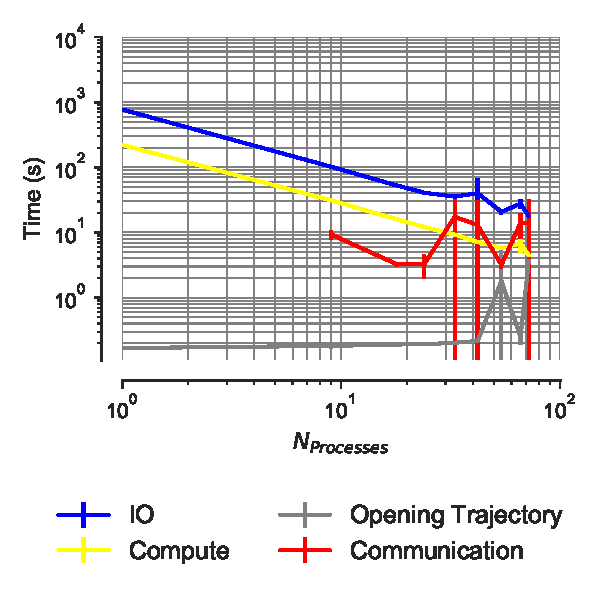
\includegraphics[width=\linewidth]{figures/main-RMSD-time_comp_IO_comparison-Bridges.pdf}
  \captionsetup{format=hang}
\caption{Scaling for different components (five repeats)}
\label{fig:ScalingComputeIO-Bridges}
\end{subfigure}
\hfill
\begin{subfigure} {.5\textwidth}
  \includegraphics[width=\linewidth]{figures/main-RMSD-BarPlot-rank-comparison_72_4-Bridges.pdf}
  \captionsetup{format=hang}
  \caption{Time comparison on different parts of the calculations per MPI rank (example)}
  \label{fig:MPIranks-Bridges}
\end{subfigure}

\caption{\emph{PSC Bridges}: Performance of the RMSD task with MPI.
Results are communicated back to rank 0 (communications included). Five independent repeats were performed to collect statistics. (a-c) The error bars show
standard deviation with respect to mean. (d) Compute \tcomp, IO \tIO, communication \tcomm, ending the for loop \text{$t_{\text{end\_loop}}$},
  opening the trajectory \text{$t_{\text{opening\_trajectory}}$}, and overheads \text{$t_{\text{overhead1}}$}, \text{$t_{\text{overhead2}}$} per MPI rank (See Table \ref{tab:notation} for the definition).
These are data from one run of the five repeats. MPI ranks 0 and 70 are stragglers. \textbf{Note:} In serial, there is no communication.}
\label{fig:MPIwithIO-Bridges}
\end{figure} 

%%%%%%%%%%%%%%%%%%

Figure \ref{fig:MPIwithIO-SuperMIC} shows performance of the RMSD task on \emph{LSU SuperMIC}. 

\begin{figure}[ht!]
\centering
\begin{subfigure}{.4\textwidth}
  \includegraphics[width=\linewidth]{figures/main-RMSD-t_total-SuperMIC.pdf}
  \caption{Scaling total (five repeats)}
  \label{fig:MPIscaling-SuperMIC}
\end{subfigure}
\hfill
\begin{subfigure}{.4\textwidth}
  \includegraphics[width=\linewidth]{figures/main-RMSD-speed_up-SuperMIC.pdf}
  \caption{Speed-up (five repeats)}
  \label{fig:MPIspeedup-SuperMIC}
\end{subfigure}
\bigskip

\begin{subfigure}{.4\textwidth}
  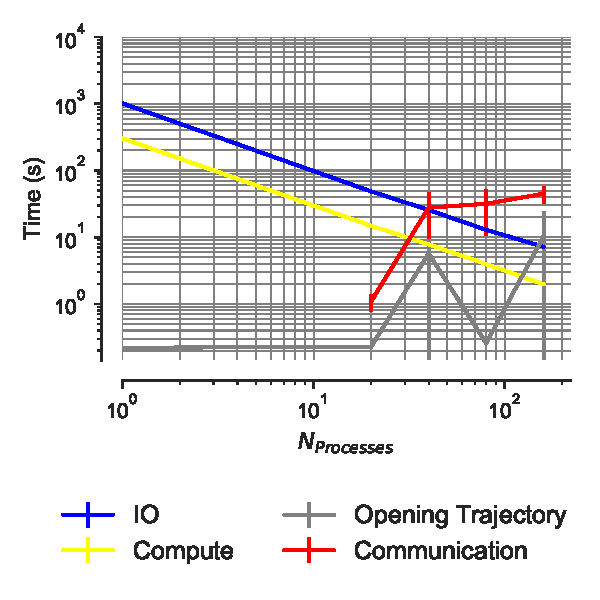
\includegraphics[width=\linewidth]{figures/main-RMSD-time_comp_IO_comparison-SuperMIC.pdf}
  \captionsetup{format=hang}
\caption{Scaling for different components (five repeats)}
\label{fig:ScalingComputeIO-SuperMIC}
\end{subfigure}
\hfill
\begin{subfigure} {.5\textwidth}
  \includegraphics[width=\linewidth]{figures/main-RMSD-BarPlot-rank-comparison_80_5-SuperMIC.pdf}
  \captionsetup{format=hang}
  \caption{Time comparison on different parts of the calculations per MPI rank (example)}
  \label{fig:MPIranks-SuperMIC}
\end{subfigure}

\caption{\emph{LSU SuperMIC}: Performance of the RMSD task with MPI.
Results are communicated back to rank 0 (communications included). Five independent repeats were performed to collect statistics. (a-c) The error bars show
standard deviation with respect to mean. (d) Compute \tcomp, IO \tIO, communication \tcomm, ending the for loop \text{$t_{\text{end\_loop}}$},
  opening the trajectory \text{$t_{\text{opening\_trajectory}}$}, and overheads \text{$t_{\text{overhead1}}$}, \text{$t_{\text{overhead2}}$} per MPI rank (See Table \ref{tab:notation} for the definition).
These are data from one run of the five repeats. MPI ranks 0 and 70 are stragglers. \textbf{Note:} In serial, there is no communication.}
\label{fig:MPIwithIO-SuperMIC}
\end{figure} 

%%%%%%%%%%%%%%%%%
Figure \ref{fig:comparison_efficiency_clusters} shows comparison of the parallel efficiency of the RMSD task between different test cases on \emph{SDSC Comet}, \emph{PSC Bridges}, and \emph{LSU SuperMIC}.  

 \begin{figure}[ht!]
\centering
\begin{subfigure}{.3\textwidth}
  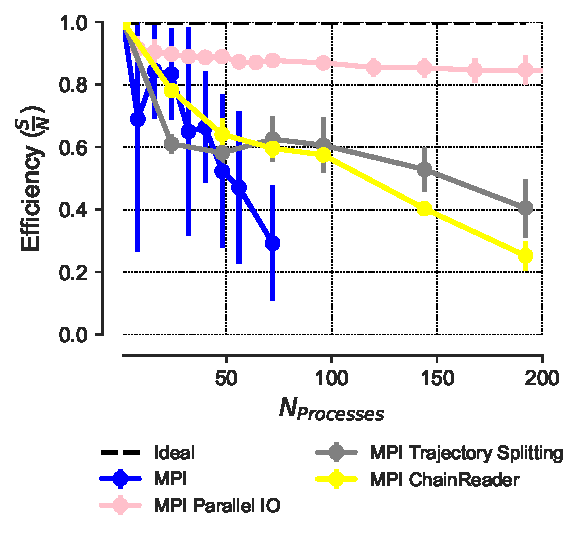
\includegraphics[width=\linewidth]{figures/Comparison_Efficiency_all_Comet.pdf}
  \caption{\emph{SDSC Comet}}
  \label{fig:comparison_efficiency}
\end{subfigure}
\hfill
\begin{subfigure}{.35\textwidth}
  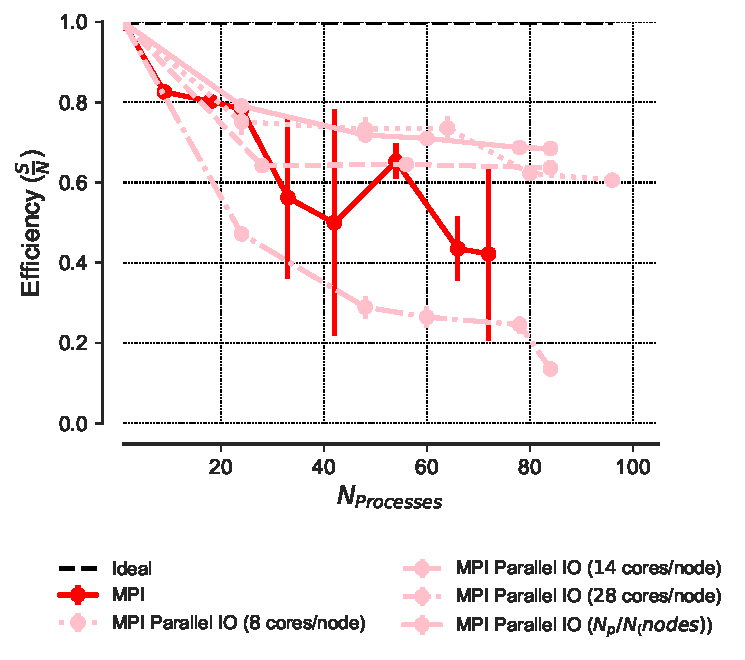
\includegraphics[width=\linewidth]{figures/Comparison_Efficiency_all_Bridges.pdf}
  \caption{\emph{PSC Bridges}}
  \label{fig:comparison_efficiency_Bridges}
\end{subfigure}
\hfill
\begin{subfigure}{.3\textwidth}
  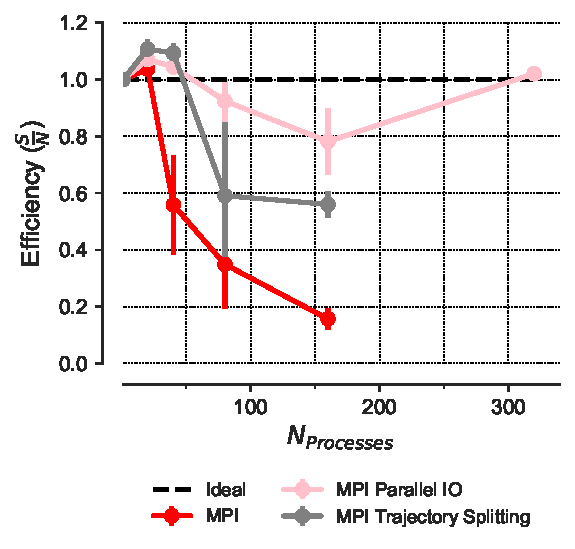
\includegraphics[width=\linewidth]{figures/Comparison_Efficiency_all_SuperMIC.pdf}
  \caption{\emph{LSU SuperMIC}}
  \label{fig:comparison_efficiency_SuperMIC}
\end{subfigure}

\caption{Comparison of the parallel efficiency between different test cases on (a) \emph{SDSC Comet}, (b) \emph{PSC Bridges}, and (c) \emph{LSU SuperMIC}.
Five repeats were performed to collect statistics and error bars show standard deviation with respect to mean.}
\label{fig:comparison_efficiency_clusters}
\end{figure} 

Figure \ref{fig:MPIwithIO-split-SuperMIC} shows how RMSD task scales with the increase in the number of cores when the trajectories are split using GA and without GA on \emph{LSU SuperMIC}.  
 
 \begin{figure}[ht!]
\centering
\begin{subfigure}{.3\textwidth}
  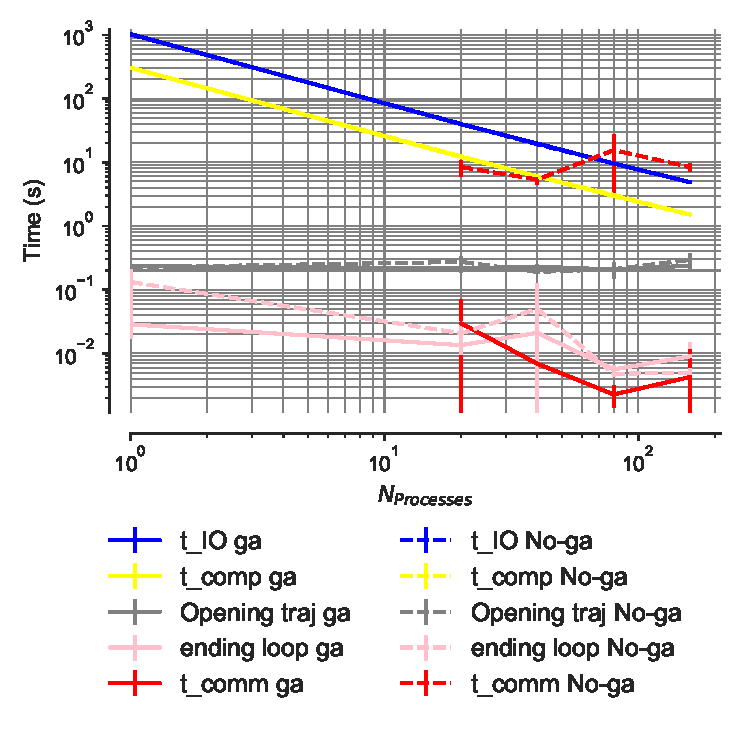
\includegraphics[width=\linewidth]{figures/Comparison_IO_compute_scaling_traj_splitting-SuperMIC.pdf}
  \captionsetup{format=hang}
  \caption{Scaling for different components}
  \label{fig:MPIscaling-SuperMIC}
\end{subfigure}
\hfill
\begin{subfigure}{.3\textwidth}
  \includegraphics[width=\linewidth]{figures/Comparison_tot_time_traj_splitting-SuperMIC.pdf}
  \caption{Scaling total}
  \label{fig:MPItottime-SuperMIC}
\end{subfigure}
\hfill
\begin{subfigure}{.3\textwidth}
  \includegraphics[width=\linewidth]{figures/Comparison_Speed_UP_traj_splitting-SuperMIC.pdf}
  \caption{Speed-up}
  \label{fig:MPIspeedup-SuperMIC}
\end{subfigure}

\caption{\emph{LSU SuperMIC}: Comparison on the performance of the RMSD task with MPI with subfiling and using either \emph{Global Arrays} for communication (``ga'') or using MPI as before (``No-ga'')  ($\RcompIO \approx 0.3$).
For \emph{Global Arrays}, all ranks update the global array (\texttt{ga\_put()}) and rank 0 accesses the whole RMSD array through the global memory address (\texttt{ga\_get()}).
Five repeats were performed to collect statistics. (a) Compute and I/O scaling versus number of processes (b) Total time scaling versus number of processes (c) Speed-up (a-c) The error bars show standard deviation with respect to mean.}
\label{fig:MPIwithIO-split-SuperMIC}
\end{figure}

